% \iffalse
\let\negmedspace\undefined
\let\negthickspace\undefined
\documentclass[journal,12pt,twocolumn]{IEEEtran}
\usepackage{cite}
\usepackage{amsmath,amssymb,amsfonts,amsthm}
\usepackage{algorithmic}
\usepackage{graphicx}
\usepackage{textcomp}
\usepackage{xcolor}
\usepackage{txfonts}
\usepackage{listings}
\usepackage{enumitem}
\usepackage{mathtools}
\usepackage{gensymb}
\usepackage{comment}
\usepackage[breaklinks=true]{hyperref}
\usepackage{tkz-euclide} 
\usepackage{listings}
\usepackage{gvv}                                        
\def\inputGnumericTable{}                                 
\usepackage[latin1]{inputenc}                                
\usepackage{color}                                            
\usepackage{array}                                            
\usepackage{longtable}                                       
\usepackage{calc}                                             
\usepackage{multirow}                                         
\usepackage{hhline}                                           
\usepackage{ifthen}                                           
\usepackage{lscape}

\newtheorem{theorem}{Theorem}[section]
\newtheorem{problem}{Problem}
\newtheorem{proposition}{Proposition}[section]
\newtheorem{lemma}{Lemma}[section]
\newtheorem{corollary}[theorem]{Corollary}
\newtheorem{example}{Example}[section]
\newtheorem{definition}[problem]{Definition}
\newcommand{\BEQA}{\begin{eqnarray}}
\newcommand{\EEQA}{\end{eqnarray}}
\newcommand{\define}{\stackrel{\triangle}{=}}
\theoremstyle{remark}
\newtheorem{rem}{Remark}
\begin{document}
\parindent 0px

\bibliographystyle{IEEEtran}
\vspace{3cm}

\title{Assignment\\[1ex]11.9.2 - 11}
\author{EE23BTECH11034 - Prabhat Kukunuri$^{}$% <-this % stops a space
}
\maketitle
\newpage
\bigskip

\renewcommand{\thefigure}{\theenumi}
\renewcommand{\thetable}{\theenumi}
\section*{Question}
Sum of the first p, q and r terms of an A.P. are a, b and c, respectively.

Prove that $\dfrac{a}{p}(q-r)+\dfrac{b}{q}(r-p)+\dfrac{c}{r}(p-q)=0$
\section*{Solution}
\begin{table}[h]
    \centering
    \begin{tabular}{|p{2cm}|p{2.80cm}|p{2.70cm}|}
    \hline
    Symbol&Value&Description\\ \hline
    $$x(n)$$&$$(x(0)+nd)u(n)$$&$$n^{th}$$ term of an A.P\\ \hline
    $$x(0)$$&$$x(0)$$&$1^{st}$ term of the A.P\\ \hline
    $$d$$&$$d$$&Common difference\\ \hline
    $$y(n)$$&$$x(n)\ast u(n)$$&Sum of n terms of an AP\\ \hline
    $$a$$&$$y(p-1)$$&Sum of first p terms of the AP\\ \hline
    $$b$$&$$y(q-1)$$&Sum of first q terms of the AP\\ \hline
    $$c$$&$$y(r-1)$$&Sum of first r terms of the AP\\ \hline
\end{tabular}
    \caption{Variable description}
    \label{tab:11.9.2.11.1}
\end{table}
\begin{align}
	x \brak{n} &\system{Z} X \brak{z} \\
    X \brak{z} &= \sum_{n=-\infty}^{\infty} x \brak{n}   z^{-n}\\
    X \brak{z} & = \sum_{n=-\infty}^{\infty}(x(0)+nd)u(n)z^{-n}\\
    u \brak{n} &\system{Z} U \brak{z} = \dfrac{1}{1-z^{-1}}, |z|>1\\
    X \brak{z} & = \dfrac{x(0)}{1-z^{-1}} + \dfrac{dz^{-1}}{(1-z^{-1})^{2}}\\
    y \brak{n} &\system{Z} Y \brak{z}\\
    Y\brak{z}&=\sum_{n=-\infty}^{\infty}y(n)z^{-n}\\
    y\brak{n}&=x\brak{n}\ast u\brak{n}\\
    Y\brak{z}&=X\brak{z}U\brak{z}\\
    Y\brak{z}&=\brak{\dfrac{x(0)}{1-z^{-1}} + \dfrac{dz^{-1}}{(1-z^{-1})^{2}}}\brak{\dfrac{1}{1-z^{-1}}}, |z|>1
 \end{align}
 By performing Z transform on Y\brak{z} using contour integration we get,
\begin{align}
    y\brak{n}&=x\brak{0}\brak{n+1}u\brak{n}+d\brak{\dfrac{{n\brak{n+1}}}{2}}u\brak{n}\\
    y\brak{n}&=\dfrac{n+1}{2}\brak{2x\brak{0}+nd}u\brak{n}\\
    a&=\dfrac{p}{2}(2x(0)+(p-1)d)\\
    b&=\dfrac{q}{2}(2x(0)+(q-1)d)\\
    c&=\dfrac{r}{2}(2x(0)+(r-1)d)
\end{align}
Back substituting values into the term $\dfrac{a}{p}(q-r)$ it can be rewritten as $\brak{\dfrac{p}{2}}\brak{\dfrac{1}{p}(q-r)(2x(0)+(p-1)d)}$

On further simplification it can be rewritten as 
\begin{align}
    \dfrac{(q-r)}{2}(2x(0)-d+pd)
\end{align}
Assuming $2x(0)-d$ as a constant $k$
\begin{align}
    \dfrac{a}{p}(q-r) = \dfrac{(q-r)}{2}(k+pd)\\
    \dfrac{(q-r)}{2}(k+pd) = \dfrac{kq+pqd-kr-prd}{2}\label{eq:31}\\
    \dfrac{(r-p)}{2}(k+qd) = \dfrac{kr+qrd-kp-pqd}{2}\label{eq:32}\\
    \dfrac{(p-q)}{2}(k+rd) = \dfrac{kp+prd-kq-qrd}{2}\label{eq:33}
\end{align}
Upon on addition of \eqref{eq:31}, \eqref{eq:32} and \eqref{eq:33} the total sum adds up to 0.
\begin{figure}[ht]
    \centering
    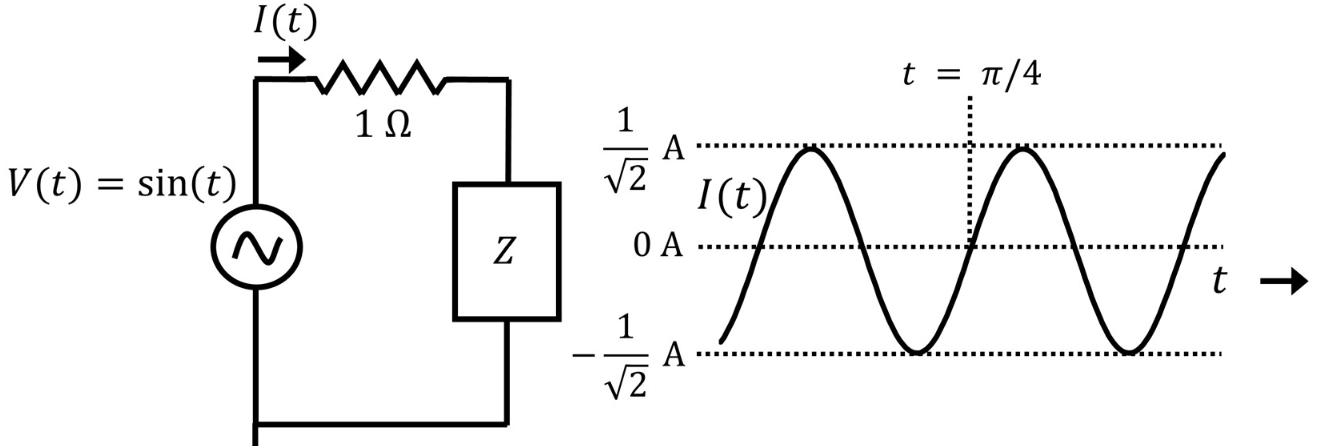
\includegraphics[width=\columnwidth]{figs/figure_1.png}
    \caption{Plot of x(n) $vs$ n}
    \label{fig:11.9.2.11.2}
\end{figure}
\begin{table}[ht]
    \centering
    \def\arraystretch{1.5}
    \begin{tabular}{|p{4.5cm}|p{4.5cm}|}
    \hline
      $$x\brak{0}$$ & $$5$$  \\ \hline
      $$d$$ & $$2$$  \\ \hline
      $$p$$ & $$8$$  \\ \hline
      $$q$$ & $$10$$  \\ \hline
      $$r$$ & $$4$$  \\ \hline
      $$a$$ & $$96$$  \\ \hline
      $$b$$ & $$140$$  \\ \hline
      $$c$$ & $$32$$  \\ \hline
\end{tabular}
    \caption{Verified Values}
    \label{tab:11.9.2.11.3}
\end{table}
\end{document}